\documentclass{article}

\usepackage[utf8]{inputenc}
\usepackage[brazilian]{babel}
\usepackage{graphicx}
\usepackage{float}
\usepackage[pdftex]{hyperref}
\usepackage{epstopdf}
\usepackage{etoolbox}
\usepackage{amsmath}
\usepackage{amsfonts}
\usepackage{amssymb}
\usepackage{caption}
\usepackage{subcaption}
\usepackage{setspace}
\usepackage{tikz}

\patchcmd{\thebibliography}{\section*}{\section}{}{}
\newcommand{\R}{\ensuremath{\mathbb{R}}}
\newcommand{\Prob}{\ensuremath{\mathbb{P}}}
\newcommand{\K}{\ensuremath{\mathbb{K}}}
\newcommand{\U}{\ensuremath{\mathbb{U}}}
\newcommand{\N}{\ensuremath{\mathbb{N}}}
\newcommand{\Lg}{\ensuremath{\mathbb{L}}}
\newcommand{\T}{\ensuremath{\rm Tr}}
\newcommand{\sg}{{\sigma(x_k)}}

\newcommand{\G}{\ensuremath{\mathcal{G}}}
\newcommand{\F}{\ensuremath{\mathcal{F}}}
\newcommand{\C}{\ensuremath{\mathcal{C}}}
\newcommand{\E}{\ensuremath{\mathcal{E}}}
\newcommand{\Hn}{\ensuremath{\mathcal{H}}}
%\newcommand{\Hoo}{\ensuremath{\mathcal{H}_\infty}}
\newcommand{\Hop}{\ensuremath{\mathcal{H}_{op}}}
% --------------------------------------------------
\newtheorem{theo}{Teorema}
\newtheorem{exa}{Exemplo}
\newtheorem{lemm}{Lema}
\newtheorem{coro}{Corolário}
\newtheorem{defn}{Definição}[section]

%opening


\begin{document}

\begin{titlepage}
\begin{center}

\newcommand{\HRule}{\rule{\linewidth}{0.5mm}}
% Upper part of the page. The '~' is needed because \\
% only works if a paragraph has started.

\includegraphics[width=0.15\textwidth]{logounicamp.pdf}~\\[1cm]

\textsc{\LARGE Universidade Estadual de Campinas}\\[1.5cm]

\textsc{\Large Faculdade de Engenharia Mecânica}\\[0.5cm]

% Title
\HRule \\[0.4cm]
{ \huge \bfseries ES828 - Laboratório de Controle de Sistemas\\ \vspace{1cm} Relatório - Experimento 2 \\
\Large{Método de identificação de plantas eletrônicas} \\[0.4cm] }

\HRule \\[1.5cm]

% Author and supervisor
\begin{minipage}{0.6\textwidth}
\begin{flushleft} \large
\emph{Nome:}\\
Daniel Dello Russo Oliveira\\ Marcelli Tiemi Kian
\end{flushleft}
\end{minipage}
\begin{minipage}{0.2\textwidth}
\begin{flushright} \large
\emph{RA}\\ 101918\\
117892
\end{flushright}
\end{minipage}

\vfill

% Bottom of the page
{\large \today}

\end{center}
\end{titlepage}


\onehalfspacing
\section{Objetivos} 
O objetivo desse experimento é realizar a identificação de parâmetros de um motor de corrente contínua com excitação independente de imãs permanentes conforme modelo proposto no roteiro\cite{bb:roteiro}. 
	
\section{Modelo matemático}
O modelo matemático do problema mostrado no esquema da figura \ref{fig:esqmotor} é dividido em duas partes: elétrica e mecânica. A primeira é mostrada na equação \ref{eq:eletrica}, com fonte de tensão V. A segunda leva em consideração o torque gerado pelo motor como $T=K_Ti$, e faz $c=\frac{r_c}{r_m}$. Aplicando a transformada de Laplace e relacionando a velocidade angular da carga com a tensão na fonte, chega-se a $G(s)$ na equação \ref{eq:gss}, onde $K=cK_T$ e $J=J_c+c^2J_m$.

\begin{figure}[H]
	\centering
	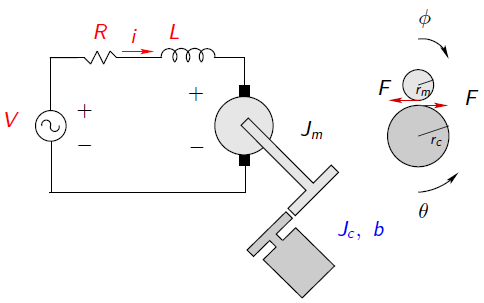
\includegraphics[width=0.8\linewidth]{esqmotor}
	\caption{Esquema do motor (elétrica e mecânica)}
	\label{fig:esqmotor}
\end{figure}

\begin{equation}
\label{eq:eletrica}
L\frac{di}{dt}+Ri=V-K_T\dot{\Phi}
\end{equation}
\begin{equation}
\label{eq:mecanica}
(J_c+c^2J_m)\ddot{\theta}+b\dot{\theta}=cK_Ti
\end{equation}
\begin{equation}
\label{eq:gss}
G(s)=\frac{\frac{K}{JL}}{s^2+(\frac{R}{L}+\frac{b}{J})s+\frac{(Rb+K^2)}{JL}}\\
\end{equation}

\section{Ensaio com motor parado}
Conforme o roteiro\cite{bb:roteiro}, ao ligar o motor com o eixo travado não geramos força contra-eletromotriz, e com isso conseguimos medir a corrente de armadura $i$ com a adição de um resistor $R_s$ como mostrado na figura \ref{fig:rotparado}. Isso nos possibilita o cálculo dos parâmetros $R [\Omega]$ e $L [H]$ pela equação \ref{eq:rotparado}.

\begin{figure}[H]
	\centering
	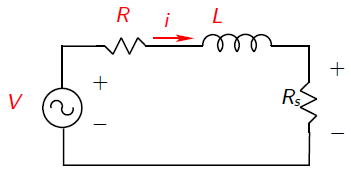
\includegraphics[width=0.8\linewidth]{rotparado}
	\caption{Circuito para motor com eixo travado}
	\label{fig:rotparado}
\end{figure}

\begin{equation}
\label{eq:rotparado}
i(t) = \frac{V_0}{(R+R_s)}(1-\exp^{-((R+R_s)/L)t})
\end{equation}

Travando o disco para impossibilitar o motor de girar seu rotor, fizemos o acionamento do módulo de potência, aguardamos a estabilização do sinal de corrente, e desligamento do sistema, obtendo a curva de corrente mostrada na figura \ref{fig:ensaiop}.

\begin{figure}[H]
	\centering
	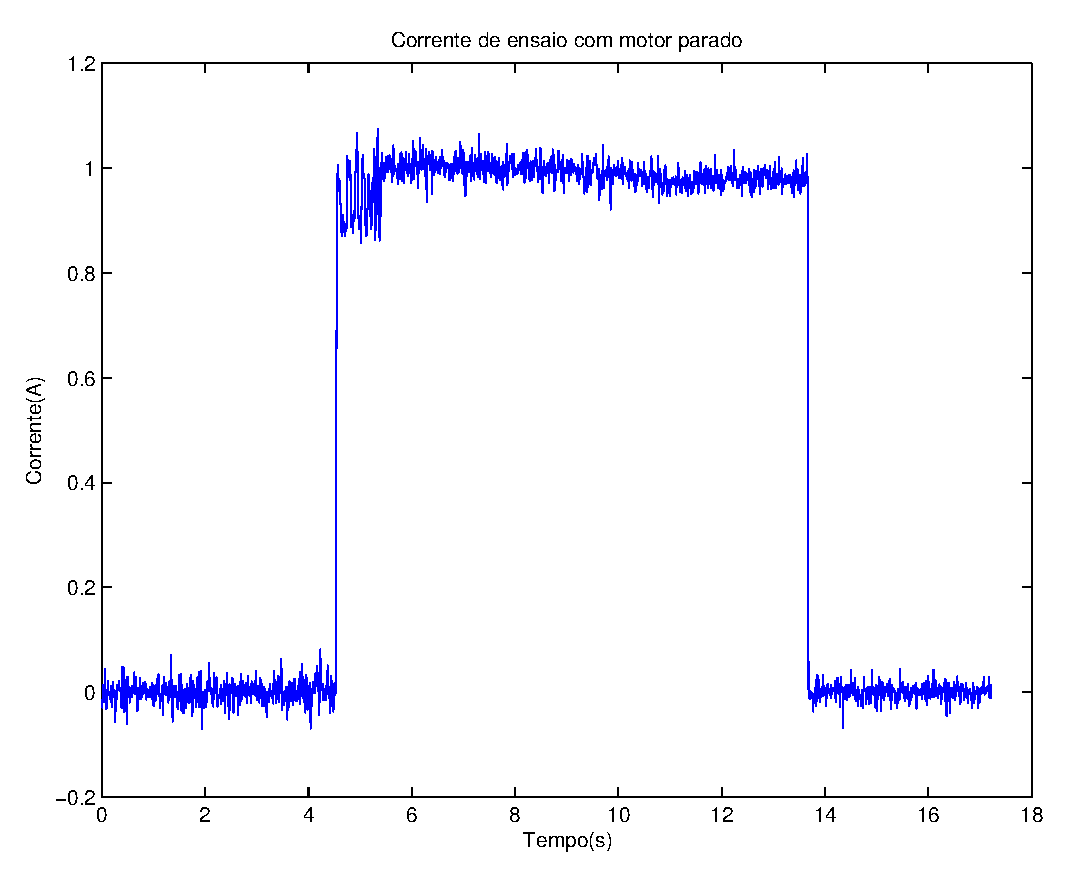
\includegraphics[width=0.8\linewidth]{../ensaiop}
	\caption{Corrente de ensaio com motor parado}
	\label{fig:ensaiop}
\end{figure}

Filtramos o sinal e destacamos alguns pontos mais relevantes para facilitar a análise, como pode ser visto na figura \ref{fig:riseI}.
\begin{figure}[H]
	\centering
	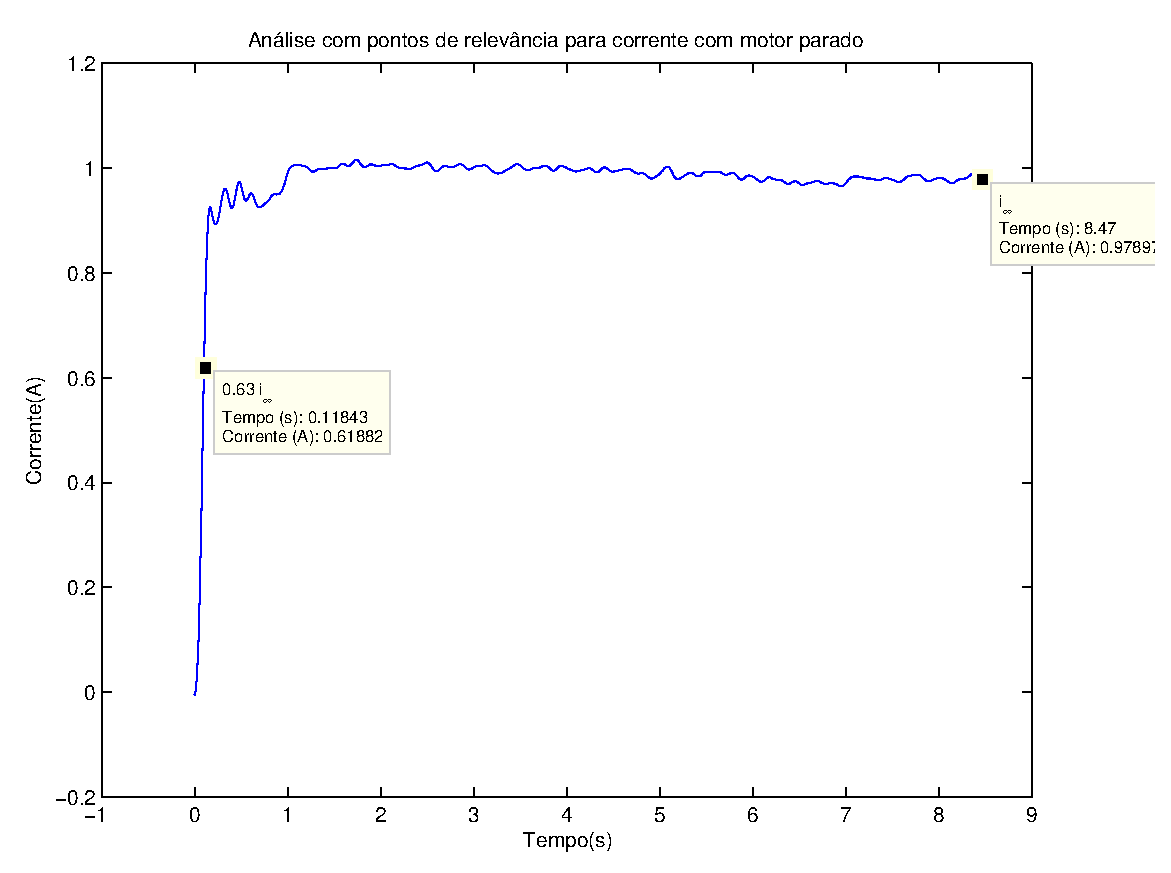
\includegraphics[width=0.8\linewidth]{../riseI}
	\caption{Pontos de relevância para corrente filtrada com motor parado}
	\label{fig:riseI}
\end{figure}

Para o cálculo do parâmetro $R$, utilizamos o valor indicado no roteiro\cite{bb:roteiro} $R_s\approxeq1 \Omega$, a tensão da fonte $V=12 V$ e a partir do momento em que a corrente se estabiliza em $i_\infty=0.9790$, calculamos seu valor conforme \ref{eq:r}.

\begin{equation}
\label{eq:r}
R = \frac{V-R_si_\infty}{i_\infty}=11.2578\Omega
\end{equation}

A indutância $L$, por sua vez, é calculada utilizando a constante de tempo da parte elétrica onde a corrente passa a ser $63\%$ do valor de regime, $i(\tau_e)=(1-\exp^{-1})i_\infty$ e portanto
$\tau_e=0.1184s$, de acordo com a equação \ref{eq:l}.

\begin{equation}
\label{eq:l}
L = \tau_e(R+R_s)=1.4516H
\end{equation}

\section{Ensaio com motor em movimento}

\section{Resultados finais}
Com todos os parâmetros necessários calculados, substituindo os valores em \ref{eq:gss}, obtemos a planta dada pela equação \ref{eq:gs}.

\begin{equation}
\label{eq:gs}
G(s)=%TODO
\end{equation}

Essa planta pode ser representada na forma de estados pela equação \ref{eq:states}, substituindo os parâmetros pelos valores calculados temos a equação \ref{eq:statesval}:
\begin{equation}
\label{eq:states}
\begin{Bmatrix}
\dot{i}\\ \dot{\nu} \\ \dot{\Theta} 
\end{Bmatrix} =
\begin{bmatrix}
-\frac{R+R_s}{L} & -\frac{K}{L} & 0\\
\frac{K}{b} & -\frac{b}{J} & 0\\
0 & 1 & 0
\end{bmatrix}
\begin{Bmatrix}
i\\ \nu \\ \Theta 
\end{Bmatrix} + 
\begin{bmatrix}
\frac{1}{L} & 0 & 0\\
\end{bmatrix}
\begin{Bmatrix}
V 
\end{Bmatrix}
\end{equation}

\begin{equation}
\label{eq:statesval}
\begin{Bmatrix}
\dot{i}\\ \dot{\nu} \\ \dot{\Theta} 
\end{Bmatrix} =
\begin{bmatrix}
-8.4441 & -0.0344 & 0\\
15.1303 & -0.0337 & 0\\
0 & 1 & 0
\end{bmatrix}
\begin{Bmatrix}
i\\ \nu \\ \Theta 
\end{Bmatrix} + 
\begin{bmatrix}
0.6889 & 0 & 0\\
\end{bmatrix}
\begin{Bmatrix}
V 
\end{Bmatrix}
\end{equation}

Com o auxílio do matlab, simulamos esse sistema a comparamos os resultados dessa simulação com os dados adquiridos durante o ensaio com o motor em movimento. Essa comparação pode ser vista nas figuras \ref{fig:simi} e \ref{fig:simv}.
\begin{figure}[H]
	\centering
	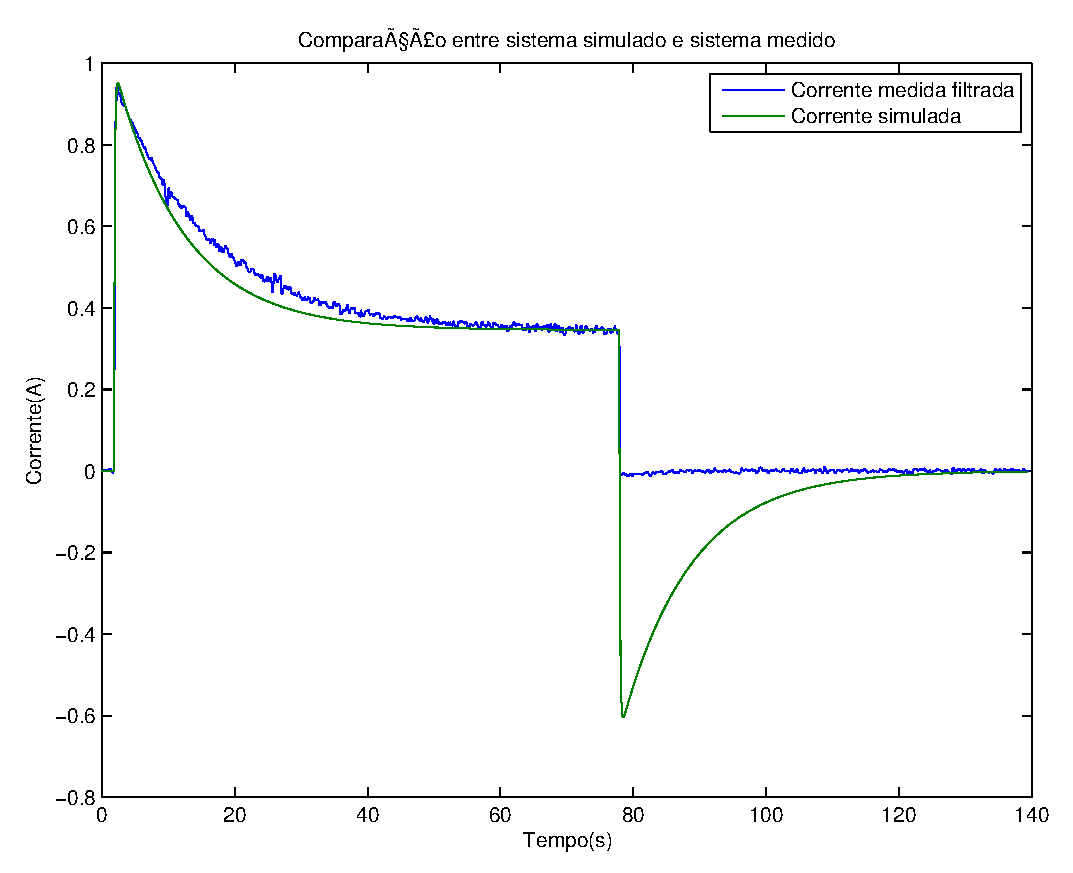
\includegraphics[width=0.8\linewidth]{../simi}
	\caption{Comparação entre corrente medida e simulada}
	\label{fig:simi}
\end{figure}
\begin{figure}[H]
	\centering
	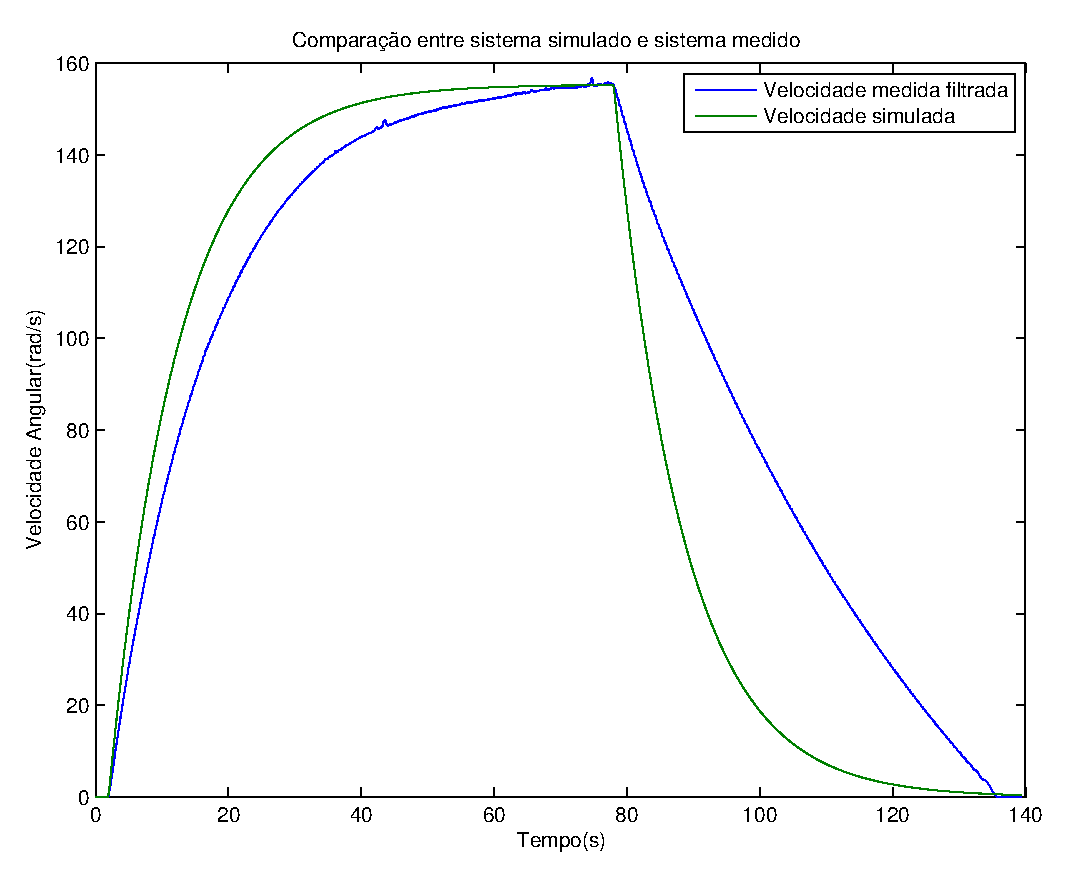
\includegraphics[width=0.8\linewidth]{../simv}
	\caption{Comparação entre velocidade angular medida e simulada}
	\label{fig:simv}
\end{figure}

A primeira coisa que notamos é que a corrente simulada apresenta um comportamento bastante diferente na queda, assumindo valores negativos. Acreditamos que o motivo dessa diferença seja a ponta H ligada no sistema, que deve se utilizar de díodos para proteger suas chaves de correntes e tensões reversas geradas pelo motor
%TODO: ANÁLISES ANÁLISES ANÁLISES ANANÁS BANANAS

\begin{thebibliography}{widestlabel}
	\bibitem{bb:roteiro}{Roteiro do experimento disponibilizado para os alunos}
\end{thebibliography}
\end{document}

